\documentclass[sigconf]{acmart}

\usepackage{booktabs} % For formal tables
\usepackage{listings}
\usepackage{amsmath} % AMS Math Package
\usepackage{amsthm} % Theorem Formatting
\usepackage{amssymb}	% Math symbols such as \mathbb
\usepackage{tikz}
\usepackage{siunitx}
\usepackage{graphicx}
\usepackage{minted} % code
\usepackage{pgfplots}
\usetikzlibrary {positioning}
\usetikzlibrary {datavisualization}

\newcommand{\curl}[1]{{\nabla} \times #1} % for curl

% Copyright
\setcopyright{none}

% DOI
\acmDOI{}

% ISBN
\acmISBN{}

%Conference
\acmConference{}{}{}

%\acmBooktitle{}
%\settopmatter{printacmref=false}

\begin{document}

\title{Simulating Turbulence with Recurrent Neural Networks }
\subtitle{}

\author{Robert Jendersie}

\maketitle

\section{Introduction}
In fluid dynamics, the behaviour of turbulence remains an unsolved problem. While the dynamics are described by the Navier-Stokes equations, a numerical simulation of sufficiently high resolution, where turbulence occurs, remains infeasible. On a statistical level however, the different scales of frequencies are known to follow the Kolmogorov energy cascade, an observation which has been used to generate turbulence with plausible energy distributions and temporal coherence \cite{kim2008wavelet}. \\
Neural networks have enjoyed success in an increasingly wide range of problems beyond classification, including long term predictions and image synthesis.
Recently, recurrent neural networks (RNNs) have been considered to predict chaotic physical systems; see \cite{vlachas2019forecasting} for a comparison off different approaches.
The possibility of having a RNN learn to simulate a turbulent flow is explored in this report.
\section{Network Architecture}
The objective of the network is to simulate the high resolution vector-field $\vec{u}$ for an arbitrary number of steps in a scene where turbulence occurs.
Instead of directly operating on $\vec{u}$, the fluid's vorticity $\zeta$
\[
\zeta = \curl{\vec{u}},
\]
is used. Assuming that $\vec{u}$ is divergence free, $\zeta$ is sufficient to reconstruct the complete vector-field. In 2D, the vorticity is a scalar-field, thus reducing the number of dimensions to operate on and making it easy to visualize.
\subsection{Inputs and Outputs}
As input, both the full $\zeta$ from the previous time step and the current state of a simulation with lower resolution with scale $s$ are considered. 
In addition, parameters describing the variable parts of the scene, such as the size of the obstacle and inflow velocity may be given.
As output, the high resolution $\zeta$ is expected.
When operating on the spatial data, a stack of convolutional layers is used to extract important features and deconvolutional layers to construct the full resolution output. Alternately, inputs and outputs can also be directly given in a frequency domain, in which case the outputs are handled by multiple dense layers of increasing size with hyperbolic tangent activations and single dense layer with linear activation at the end to match the correct output size.\\
 Since tensorflow has limited support for complex numbers, real and imaginary parts are separated into two float channels.
\subsection{Recurrent Layers}
\begin{figure}
	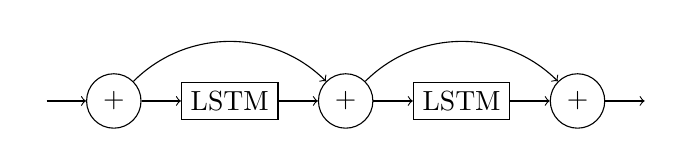
\begin{tikzpicture}
	[align=center,node distance=0.5cm, add/.style={circle,draw},layer/.style={rectangle,draw},placeholder/.style={}]
	\node[placeholder] (input) {};
	\node[add] (add2) [right=of input] {+};
	\node[layer] (rnn0) [right=of add2] {LSTM};
	\node[add] (add0) [right=of rnn0] {+};
	\node[layer] (rnn1) [right=of add0] {LSTM};
	\node[add] (add1) [right=of rnn1] {+};
	\node[placeholder] (rnn2) [right=of add1] {};
	\draw [->] (input.east) -- (add2.west);
	\draw [->] (add2.east) -- (rnn0.west);
	\draw [->] (add2) to [bend left=45] (add0);
	\draw [->] (rnn0.east) -- (add0.west);
	\draw [->] (add0.east) -- (rnn1.west);
	\draw [->] (add0) to [bend left=45] (add1);
	\draw [->] (rnn1.east) -- (add1.west);
	\draw [->] (add1.east) -- (rnn2.west);
	\end{tikzpicture}
	\caption{Residual Layers.}
	\label{residualLayers}
\end{figure}
The main work is done by the recurrent layers, for which both Long Short-Term Memory(LSTM) and Gated Recurrent Units(GRU) are suitable. Where dimensions are compatible, residual connections are inserted, adding together the inputs and outputs of the current layer as shown by Figure~\ref{residualLayers}. The idea is that the task of learning just modifications instead of the full mapping is simpler. This generally improves the training success, especially for longer networks, at low costs for both training and execution since no extra weights are needed and tensor addition operations are cheap \cite{he2016deep}. \\
An important parameter of the recurrent layers is their state-fullness. Usually RNNs are fed a fixed number of steps to predict the next step, after which the internal memory of each unit is reset to $0$. For a simulation, processing just one time step should yield the next one. Also, the training can impose some practical limits on the number of time steps given as input, which may be shorter than some long term dependencies in the data. Thus, only state-full networks are considered here.
%todo refs
%%%%%%%%%%%%%%%%%%%%%%%%%%%%%%%%%%%%%%%%%%%%%%%%%%%%%%%%%%%%%%%%%%%%%%%%%%%%%%%
\section{Training Setup}\label{sec:training}
\begin{figure}
	\begin{tikzpicture}
	\node[anchor=south west,inner sep=0] (image) at (0,0) {\includegraphics[width=0.45\textwidth]{imgs/scene.png}};
	\begin{scope}[x={(image.south east)},y={(image.north west)}]
		\draw[blue,ultra thick] (0.0,0.419) rectangle (0.05,0.581) node[above] {source};
		\draw[blue,ultra thick] (0.2,0.5) ellipse [x radius=0.05, y radius=0.1] (0.2,0.6) node[above] {obstacle};
	\end{scope}
	\end{tikzpicture}
	\caption{The Scene.}
	\label{trainingScene}
\end{figure}
The training setup, as shown rotated by $\ang{90}$ in Figure~\ref{trainingScene}, consists of a source at the bottom, where smoke flows in and a circular obstacle above it. Through buoyancy, the smoke flows around the obstacle on both sides, causing turbulence in the area above when the streams merge. To add some variation, noise is applied to the inflow. Also the obstacle size can be changed and some random initial velocity may be applied to the input.
Advection is computed with a second order semi Lagrangian scheme.\\
The low resolution inputs for the purpose of training are extracted from the 2D discrete Fourier Transform 
\[
Z = \mathcal{F} (\zeta),
\]
which is also depicted in Figure~\ref{lowFreqs}.
Since $\zeta$ is real, symmetries in $Z$ allow the use of only the upper quadrants. The resulting real part is even $Z(u,v)=Z(-u,-v)$ and the imaginary part odd $Z(u,v)=-Z(-u,-v)$. The input consists of all frequencies up to $s$, the expected output of all larger frequencies.
\begin{figure}
	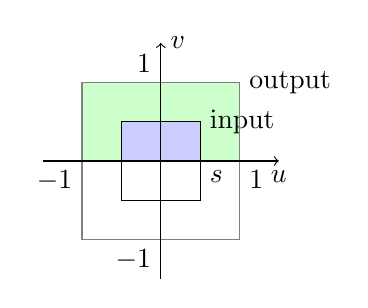
\begin{tikzpicture}
	\draw[fill=green!20] (-1.0,0.0) rectangle (1.0,1.0) node[right] {output};
	\draw[fill=blue!20] (-0.5,0.0) rectangle (0.5,0.5) node[right] {input};
	\draw (-0.5,-0.5) rectangle (0.5,0.5);
	\draw (-0.5,-0.5) rectangle (0.5,0.5);
	\draw[thin, gray] (-1.0,-1.0) rectangle (1.0,1.0);
	\draw[->] (-1.5,0) -- (1.5,0) node[below] {$u$};
	\draw[->] (0,-1.5) -- (0,1.5) node[right] {$v$};
	\draw(-1.0,0.0) node[below left] {$-1$} (1.0,0.0) node[below right] {$1$};
	\draw(0.0,-1.0) node[below left] {$-1$} (0.0,1.0) node[above left] {$1$};
	\draw(0.5,0.0) node[below right] {$s$};
	\end{tikzpicture}
	\caption{Input and outputs from $Z(u,v)$.}
	\label{lowFreqs}
\end{figure}
As optimizer, RMSprop with default arguments \cite{RMSprop} is used. Other options such as stochastic gradient descent and Adam where briefly considered but seem to perform worse. As loss functions, the mean square error 
\begin{equation}\label{eq:mse}
	\frac{1}{n_s}\sum_{x}\sum_{y} (\zeta(x,y) - \hat{\zeta}(x,y))^2,
\end{equation}\label{eq:ferr}
for spatial outputs and
\begin{equation}
\frac{1}{n_f}\sum_{u}\sum_{v} |Z(u,v) - \hat{Z}(u,v)|^2,
\end{equation}
for frequency outputs are taken.\\
Instead of a fixed size data set, the generator pattern is used. The numerical simulation can provide a continuous stream of new data, minimizing the risk of over-fitting. Also, common data preprocessing such as shuffling and batching after each epoch pose problems with the persistent state of the network over multiple training steps.
\subsection{Stateful Recurrent Neural Networks}
As mentioned before, RNN layers use a special training process displayed in Figure~\ref{rnnTraining}. Instead of passing through one sample and back propagating the error, $k$ time steps are processed by a loop and only the final output is forwarded to the error computation. During back propagation, the loop is unrolled, effectively stacking the same layer multiple times. 
\begin{figure}
	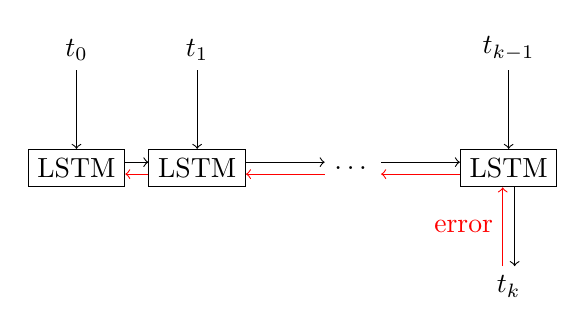
\begin{tikzpicture}
	[gap/.style={},layer/.style={rectangle,draw}, error/.style={red}]
	\node[gap]   (inp0) {$t_0$};
	\node[gap]   (inp1) [right=of inp0] {$t_1$};
	\node[layer] (rnn0) [below=of inp0] {LSTM};
	\node[layer] (rnn1) [right=of rnn0, below=of inp1] {LSTM};
	\node[gap]   (rnn2) [right=of rnn1] {$\dots$};
	\node[layer] (rnn3) [right=of rnn2] {LSTM};
	\node[gap]   (inp2) [right=of inp1, above=of rnn3] {$t_{k-1}$};
	\node[gap]   (outp) [below=of rnn3] {$t_k$};
	\draw [->] (inp0.south) -- (rnn0.north);
	\draw [->] (inp1.south) -- (rnn1.north);
	\draw [->] (inp2.south) -- (rnn3.north);
	\draw[transform canvas={yshift=0.5ex},->] (rnn0.east) -- (rnn1.west);
	\draw[transform canvas={yshift=-0.5ex},error,->](rnn1.west) -- (rnn0.east); 
	\draw[transform canvas={yshift=0.5ex},->] (rnn1.east) -- (rnn2.west);
	\draw[transform canvas={yshift=-0.5ex},error,->](rnn2.west) -- (rnn1.east); 
	\draw[transform canvas={yshift=0.5ex},->] (rnn2.east) -- (rnn3.west);
	\draw[transform canvas={yshift=-0.5ex},error,->](rnn3.west) -- (rnn2.east); 
	\draw[transform canvas={xshift=0.5ex},->] (rnn3.south) -- (outp.north);
	\draw[transform canvas={xshift=-0.5ex},error,->](outp.north) -- node[auto] {error} (rnn3.south); 
	\end{tikzpicture}
	\caption{A single LSTM layer in training.}
	\label{rnnTraining}
\end{figure}
While a larger window size $k$ may allow the network to pick up long term dependencies, the increased training time sets practical bounds and the impact of different choices is tested.\\
Processing multiple samples together as a batch and updating weights from the accumulated error is important both to speed up the training and to prevent over-fitting. However, for state-full networks, continuity across batches is required. Thus, batches of size $b$ would need to be build from $b$ different time-series. Instead of running multiple simulations a ring buffer of previous steps is kept. By choosing a sufficient distance $d$, a history of size $b \cdot d$ can be used to create batches of seemingly independent simulations. Let $p$ be the pointer to the current position of the ring buffer. Then after just one simulation step the next batch is constructed from the elements with indices
\[
ind_i = (p + i \cdot d) \mod (b \cdot d),
\]
where $i=0,\dots,b-1$.
Since tensorflow requires for state-full RNNs that the batch size is a fixed parameter, the trained model is impractical for the actual use case where just one time series should be simulated. Fortunately this issue, as well as the awkwardness of having to input multiple time steps to receive just one output, can be circumvented by building another model with the same architecture but $b=k=1$. Then the training results from \textit{modelT} can be transferred to \textit{modelP} via 
\begin{minted}{python}
	modelP.set_weights(modelT.get_weights())
\end{minted}
\section{Evaluation}
Quality of the different networks is evaluated on validation sets of size $1024$ generated with the same setup as the training process, but varying seeds for the random number generator.
\subsection{Network Objective}\label{sec:eva:objective}
\begin{figure}
	\begin{tikzpicture}
	\begin{axis}[ymode=log, legend pos = south east, xlabel=timesteps $t$, ylabel=$(\zeta - \hat{\zeta})^2$]
	\addplot+[mark size=1pt] table[x=t, y=FullRes, col sep=comma]{data/fullres.csv};
	\addlegendentry{FullRes}
	\addplot+[mark size=1pt] table[x=t, y=Conv, col sep=comma]{data/fullres.csv};
	\addlegendentry{Conv}
	\addplot+[mark size=1pt] table[x=t, y=LowFreq, col sep=comma]{data/fullres.csv};
	\addlegendentry{LowFreq}
	\end{axis}
	\end{tikzpicture}
	\caption{Error over time for different approaches.}
	\label{objectiveError}
\end{figure}
First, we take a look at two different possible objectives. Either to perform the full simulation where the outputs are fed back as input for the next step, or to generate details from a lower frequency simulation.
In Figure~\ref{objectiveError} the mse for these approaches is shown, with the addition of a purely convolutional network without recurrent units for the former approach. Unsurprisingly, the full resolution networks perform better initially, since they mostly have to reproduce the input. However, the outputs quickly diverge from the expected results until settling in a stable loop.
\begin{figure}
	\includegraphics[width=0.5\textwidth]{imgs/fullres_series.png}
	\caption{Closed loop network after 1, 8, 32, 64 steps.}
	\label{closedLoop}
\end{figure}
A closer look at the outputs of FullRes in Figure~\ref{closedLoop} shows that while some major features of the scene are preserved, details are lost and artefacts have formed. On the other hand, the upscaling approach improves for over 40 steps while filling its internal memory and then continues to produce approximation of the expected state. Thus, in following experiments we attempt to improve on the second approach.
\subsection{Frequency and Spatial IO}
To compare spatial(S) and frequency(F) inputs/outputs, the same inner RNN is combined with appropriate outer processing. Since these additional layers can have a significant impact on the achieved quality, network with similar execution times are considered. In Table~\ref{tab:freqIO}, average times for a single step are shown in addition to the average errors \eqref{eq:mse} and the square root of \eqref{eq:ferr}.
\begin{table}
\centering
\caption{Error for different IO approaches.}
\label{tab:freqIO}
\begin{tabular}{lccc}
	\hline
	    & S error & F error & t in s \\ \hline
	input           & 0.0277 & 7.9214 & 0.0000 \\
	S$\rightarrow$S & 0.0077 & 4.6925 & 0.0046 \\
	F$\rightarrow$S & 0.0081 & 4.7448 & 0.0045 \\
	F$\rightarrow$F & 0.0080 & 4.3151 & 0.0037 \\
	S$\rightarrow$F & 0.0074 & 4.1384 & 0.0037 \\ \hline
\end{tabular}
\end{table}
All variants minimize both error measures to a certain extend, when compared to the upscaled input.
From these aggregate values it does seem howver, like extracting relevant features works better from the spatial view. For the outputs, expecting frequency leads to far better frequency results and similar spatial error.
A more detailed look at the power spectrum summed up over the v-axis in Figure~\ref{powerspectrum} and averaged over a whole validation set, reveals that both output variants manage to reproduce some details across all frequencies. However, the deconvolutional versions exhibit larger deviations in higher frequencies.
\begin{figure}
	\includegraphics[width=0.5\textwidth]{imgs/powerspectrum.pdf}
	\caption{Power spectrum of different IO approaches.}
	\label{powerspectrum}
\end{figure}
\subsection{Network Size}
How the size of the recurrent layers impacts the results is explored in Table~\ref{tab:size}. Both the number of layers and the size of each unit have only minor effects and diminishing returns. Going from $1$ layer to $5$ layers decreases the measured spatial error by just $2.5\%$ and from $3$ to $5$ the frequency error does not improve at all.
Similar observations are made for the unit size, where going from $40$ to $120$ gives a $5\%$ improvement in spatial error while the difference from $80$ to $120$ is only $1\%$.
\begin{table}
	\centering
	\caption{Size variations of the recurrent layers.}
	\label{tab:size}
	\begin{tabular}{lccccc}
		\hline
		      & layers & unit size & S error & F error & t in s \\ \hline
		Len1  &   1    &    80     & 0.0077  & 4.2271  & 0.0037 \\
		Len2  &   3    &    80     & 0.0076  & 4.1755  & 0.0042 \\
		Len3  &   5    &    80     & 0.0075  & 4.1773  & 0.0046 \\
		Size1 &   3    &    40     & 0.0079  & 4.2675  & 0.0040 \\ 
		Size3 &   3    &    120    & 0.0075  & 4.1768  & 0.0042 \\ \hline
	\end{tabular}
\end{table}
\subsection{Window and Batch Size}
To determine the impact of training parameters on the success, we train the same model architecture for $50$ epochs on the same simulation but organize the data with varying window(w)- and batch(b)-sizes. How the loss on the validation set changes, is plotted in Figure~\ref{bwsize}.
\begin{figure}
	\begin{tikzpicture}
	\begin{axis}[legend style={at={(1.05,1.0)}, anchor=north}, xlabel=epochs $t$]
	\addplot+[mark size=1pt] table[x=epoch, y=W1B1, col sep=comma]{data/wbsize.csv};
	\addlegendentry{1 1}
	\addplot+[mark size=1pt] table[x=epoch, y=W1B32, col sep=comma]{data/wbsize.csv};
	\addlegendentry{1 32}
	\addplot+[mark size=1pt] table[x=epoch, y=W4B4, col sep=comma]{data/wbsize.csv};
	\addlegendentry{4 4}
	\addplot+[mark size=1pt] table[x=epoch, y=W8B4, col sep=comma]{data/wbsize.csv};
	\addlegendentry{8 4}
	\addplot+[mark size=1pt] table[x=epoch, y=W16B4, col sep=comma]{data/wbsize.csv};
	\addlegendentry{16 4}
	\addplot+[mark size=1pt] table[x=epoch, y=W16B16, col sep=comma]{data/wbsize.csv};
	\addlegendentry{16 16}
	\end{axis}
	\end{tikzpicture}
	\caption{Frequency error during training with inputs (w b).}
	\label{bwsize}
\end{figure}
To have the recurrent layers learn anything meaningful, windows of size larger than $1$ seem necessary. Both (1 1) and (1 32) show no improvement after the initial epoch, while (4 4) has an overall down trend. Further increasing the size to (8 4) or even (16 4) lead to even better results, but with diminishing returns. Also, the training time per epoch increases by more than $50\%$, as shown in Table~\ref{tab:bwsize}.\\
For the other parameter, mini batches of size $4$ help prevent overhitting due to similarity of the consecutive time steps. Furthermore, a larger batch size leads to convergence in fewer epochs at no cost to the quality of the result. Since back-propagation takes the majority of the time during the training process, as seen by a duration increase of less than $1\%$ from (16 4) to (16 16), this is also huge practical advantage in terms of training time required. With our training setup however, the time it takes to fill the data buffer is proportional to $w*b$, which imposes an upper bound to the possible speedup.
\begin{table}
	\centering
	\caption{Training times depending on batch- and window size.}
	\label{tab:bwsize}
	\begin{tabular}{ccc}
		\hline
		window  & batch  & t in ms \\ \hline
		1  & 32 &   53    \\
		4  & 4  &   154   \\
		8  & 4  &   232   \\
		16 & 4  &   370   \\
		16 & 16 &   373   \\ \hline
	\end{tabular}
\end{table}
\subsection{Additional Inputs}
* overall worse performance
* loss of details?
* providing additional inputs can mitegrate to some extend
\section{Conclusion}
\subsection{Limitations}
* preserving sufficient details since state is too small
* producing full resolution frequency too many weights since similarity can not be used
* computing time should be lower than the numerical simulation
\subsection{Future Work}
* convlstm
* tilebased
* combine \ref{sec:eva:objective}

\bibliographystyle{ieeetr}
%\bibliographystyle{ACM-Reference-Format}
%\nocite{*}
\bibliography{references}
\end{document}
